\documentclass[11pt]{article}

\usepackage[utf8]{inputenc}
\usepackage[francais]{babel}
\usepackage{graphicx}
\usepackage{wrapfig}
\usepackage{fullpage}

\usepackage[top=100pt,bottom=70pt,left=60pt,right=60pt]{geometry}

\usepackage{amsfonts,amssymb,amsmath,amsthm} 
\usepackage[colorlinks,urlcolor=blue,linkcolor=black,citecolor=gray]{hyperref}

\usepackage{tikz}


\newtheoremstyle{exostyle}
{\topsep}% espace avant
{}%{\topsep}% espace apres
{}% Police utilisee par le style de thm
{}% Indentation (vide = aucune, \parindent = indentation paragraphe)
{\bfseries}% Police du titre de thm
{.}% Signe de ponctuation apres le titre du thm
{ }% Espace apres le titre du thm (\newline = linebreak)
{\thmname{#1}\thmnumber{ #2}\thmnote{. \normalfont{\textit{#3}}}}% composants du titre du thm : \thmname = nom du thm, \thmnumber = numéro du thm, \thmnote = sous-titre du thm

\newtheoremstyle{exostyle*}
{\topsep}% espace avant
{}%{\topsep}% espace apres
{}% Police utilisee par le style de thm
{}% Indentation (vide = aucune, \parindent = indentation paragraphe)
{\bfseries}% Police du titre de thm
{.}% Signe de ponctuation apres le titre du thm
{ }% Espace apres le titre du thm (\newline = linebreak)
{\thmname{#1}\thmnote{. \normalfont{\textit{#3}}}}% composants du titre du thm : \thmname = nom du thm, \thmnumber = numéro du thm, \thmnote = sous-titre du thm


\newcommand{\R}{\ensuremath{\mathbb R}}
\newcommand{\PP}{\ensuremath{\mathbb P}}
\newcommand{\CC}{\ensuremath{\mathbb C}}
\newcommand{\N}{\ensuremath{\mathbb N}}
\newcommand{\ZZ}{\ensuremath{\mathbb Z}}
\newcommand{\ds}{\displaystyle}
\newcommand{\Mm}{\mathcal{M}}
\renewcommand{\Im}{{\mathrm{Im} \, }}
\newcommand{\bR}{\mathbb R}
\newcommand{\bN}{\mathbb N}
\DeclareMathOperator{\tr}{\mathrm{Tr}}

\theoremstyle{exostyle}
\newtheorem{exercice}{Exercice} 
\newtheorem{solution}{Solution}

\usepackage{titlesec}
\renewcommand{\thesection}{\Roman{section}}
\titleformat{\section}[display]
{\large\bfseries}
{\vspace{.5cm}\titlerule[1.pt]}
{-10pt}
{\filright \large \qquad \thesection\ \large\bfseries\filright}[{\vspace{1.5mm}\titlerule[1pt]\vspace{5mm}}]


\newcommand{\ZeroRoman}[1]{% 0 + \Roman
  \ifcase\value{#1}\relax 0\else% Chapter 0
  \Roman{#1}\fi}% All other chapters
\renewcommand{\thesection}{\ZeroRoman{section}}

\date{} 
\author{}


%#############################################################################################
\begin{document}
\selectlanguage{french}


\noindent 
Sorbonne Universit\'e - Université Paris Cité     \hfill   Ann\'ee 2023-2024 \\
Pr\'eparation \`a  l'agr\'egation        \hfill     Vendredi 29 mars 2024 \\ % \emph{Dur\'ee : 3h}
 %\hfill \emph{Calculatrices et t\'el\'ephones interdits} \\
\noindent {\rule{\textwidth}{.2mm}}\\[-5mm]
\begin{center}
{\large \textsc{Examen option B} }\\[-5mm]
\end{center}
\noindent {\rule{\textwidth}{.2mm}}\\[1cm]

L’examen comporte deux exercices indépendants.

{\bfseries Merci de r\'ediger les deux exercices sur deux copies s\'epar\'ees.}

\begin{exercice}
Dans cet exercice, on s’intéresse au système différentiel suivant 
\begin{equation} \label{proiepred}
\left\{ 
\begin{aligned}
x' &= x(1  -y) \\
y' &= y(- 1 +x). \\
\end{aligned} 
\right.
\end{equation}
A l'instant initial, on suppose que $(x(0), y(0))=(x_0 , y_0 )$ avec $x_0 > 0$ et $y_0 > 0$.
\begin{enumerate}
  \item  Discuter l'existence et l'unicité de solution au système  \eqref{proiepred}.
  \item Montrer que, pour $x_0 > 0$  et $y_0 > 0$ donnés, la solution maximale vérifie $x(t) > 0$ et $y(t) > 0$ pour tout $t$ dans son intervalle
de définition. 
  \item Soit $H(\tilde{x}, \tilde{y}) := \tilde{y}+\tilde{x} -\ln(\tilde{y}) - \ln(\tilde{x})$. Montrer que $ t \mapsto H(x(t),y(t))$ est constante où $x,y$ sont les solutions maximales du système~\eqref{proiepred}. 
\item A l'aide de la question précédente, montrer que $x$ et $y$ sont bornées. En déduire que les solutions sont définies sur $\bR$.

\item Dans cette question, nous allons tracer le portrait de phase du système différentiel~\eqref{proiepred}.
\begin{enumerate}
  \item Donner les points stables de~\eqref{proiepred}.
  \item Calculer les isoclines de~\eqref{proiepred}.
  \item Dessiner un portrait de phase.
  \item  En utilisant le portrait de phase de  \eqref{proiepred}, montrer que les solutions parcourent successivement les 4 zones délimitées par les isoclines. (il n’est pas nécessaire de justifier tous les cas possibles)
  \item En utilisant que $t \mapsto H(x(t),y(t))$ est constante, montrer que les solutions sont périodiques.
\end{enumerate}

\end{enumerate}
\end{exercice}




%%%%%%%%%%%%%%%%%%%%%%%%%%%%%%%%%%%%%%%%%%%%%%%%%%% 

\newpage

\begin{exercice}
  Soient $n$ un entier non nul, $A\in \Mm_{n}(\bR)$ une matrice réelle symétrique et $S\in \Mm_{n}(\bR)$ une matrice réelle symétrique définie-positive. 
  On note $\langle \cdot, \cdot \rangle$ le produit scalaire euclidien sur $\bR^n$ et $\|x\|^2 = \langle x,x \rangle$ la norme associée.
  %On note $I_n$ la matrice identité de $\Mm_n(\bR)$.
  
  On s'intéresse au problème d’optimisation sous contrainte 
  \begin{equation}
    \label{eq:optim_contrainte}
    \min_{x \in \bR^n, g(x) = 1} f(x)  
  \end{equation}
  où la fonction $f:\bR^n \rightarrow \bR$ définie par
$f(x) = \frac{1}{2} \langle x, A x \rangle $
et la contrainte $g:\bR^n \rightarrow \bR$ est donnée par $g(x) =\frac{1}{2} \langle x, S x \rangle $. \\
  
\begin{enumerate}
  \item Montrer que le problème d’optimisation sous contrainte~\eqref{eq:optim_contrainte} a une solution.
  
  \emph{Indication :} on pourra montrer que l’ensemble $\lbrace x \in \bR^n, g(x) = 1 \rbrace$ est compact.
\end{enumerate}

\medskip

{\bf I. Caractérisation de la solution}

\begin{enumerate}
\setcounter{enumi}{1}
 \item \label{q:calcul-gradient_1} 
 Calculer le gradient de $f$ et celui de $g$ et montrer que
$$
\nabla f(x) = A x \qquad \mbox{et} \qquad \nabla g(x) =  Sx.
$$
  %
  \item Donner une condition nécessaire pour que $x_* \in \bR^n$ soit une solution du problème d’optimisation sous contrainte~\eqref{eq:optim_contrainte} grâce aux multiplicateurs de Lagrange. 
  %
  \item 
  Soit $L \in \Mm_n(\bR)$ le facteur de la décomposition Cholesky de $S$. 
  On rappelle que $L$ est une matrice inversible triangulaire inférieure vérifiant $L^T L = S$.

  Montrer que l’équation d’Euler Lagrange peut se réécrire 
  \[
    B x_* = \lambda x_*,  
  \]
  où $B$ est une matrice que l’on donnera en fonction de $A$ et $L$.
  %Montrer que si $A$ est injective alors $f$ admet  un unique minimiseur global. Dans ce cas, exprimer le minimiseur global.
  %
  \item Montrer que la solution $x_*$  du problème d’optimisation sous contrainte~\eqref{eq:optim_contrainte} est un vecteur propre associé à la plus petite valeur propre de la matrice $B$.
\end{enumerate}  

{\bf II. Approximation du minimiseur} \\
Pour $\mu>0$, soit $J_\mu : \bR^n \to \bR$ la fonction définie par 
\[
  J_\mu(x) = f(x) + \mu g(x) =  \frac{1}{2} \langle x, A x \rangle + \frac{\mu}{2} (\langle x, S x \rangle-1)^2.
\]

Soit $x_*$ une solution du problème d’optimisation~\eqref{eq:optim_contrainte}.

%On suppose désormais que le problème  d’optimisation sous contrainte~\eqref{eq:optim_contrainte} admet une unique solution $x_*$.

On cherche à approcher $x_*$ par le problème de minimisation 
\begin{equation}
  \label{eq:penalisation}
  \min_{x \in \bR^n} J_\mu(x).
\end{equation}
%
\begin{enumerate}
\setcounter{enumi}{5}
%
  \item Montrer que $J_\mu$ est coercive.
  

  \emph{On rappelle que $F : \bR^n \to \bR$ est coercive si $\lim_{\|x\| \to \infty} F(x) = \infty$}

  \item Montrer que le problème de minimisation~\eqref{eq:penalisation} a une solution.
  
  \item Soit $x_\mu$ une solution du problème~\eqref{eq:penalisation}. Montrer que $J_\mu(x_\mu) \leq J(x_*)$.

  \item Soit $(\mu_n)_n$ une suite telle que $\lim\limits_{n \to \infty} \mu_n = \infty$.
  En déduire que $(x_{\mu_n})_{n}$ est compacte et qu’il existe une valeur d’adhérence $\overline{x}$.

  \item Pour $\mu>0$, soit $x_\mu$ une solution du problème de minimisation~\eqref{eq:penalisation}.
  Pour $(\mu_n)_n$ une suite telle que $\lim\limits_{n \to \infty} \mu_n = \infty$, soit $\overline{x}$ une valeur d’adhérence de $(x_{\mu_n})_n$.
  On note $p(x) =  (\langle x, S x \rangle-1)^2.$

  Soit $0 < \mu < \nu$.
  \begin{enumerate}
    \item Montrer que 
    \[
      J_{\mu}(x_\mu) \leq  J_{\mu}(x_{\nu}), \quad \text{ et } \quad J_{\nu}(x_\nu) \leq  J_{\nu}(x_{\mu}).
    \]
    \item En déduire que $(\nu - \mu) (p(x_\mu)-p(x_\nu)) \geq 0$ et que $\mu \mapsto p(x_\mu)$ est décroissante.
    En utilisant la question 8, montrer que $p(\overline{x}) = 0$.
    \item En déduire que $\overline{x}$ est une solution du problème d’optimisation sous contrainte~\eqref{eq:optim_contrainte}.
  \end{enumerate}
\end{enumerate}
\end{exercice}



% #############################################################################################
\newpage

\noindent {\rule{\textwidth}{.2mm}}\\[-5mm]
\begin{center}
{\large \textsc{Corrigé examen option B} }\\[-5mm]
\end{center}
\noindent {\rule{\textwidth}{.2mm}}\\[1cm]

\section*{Correction exercice EDO}

\begin{solution}
  \begin{enumerate}
    \item Cauchy-Lipschitz local.
    \item si $x$ devient négatif, alors par continuité il existe $t$ tel que $x(t) = 0$. Or $x = 0$ est solution sur $\bR$ du problème de Cauchy avec $x(t)=0$.
    \item Calcul direct.
    \item Par 2., $x$ ou $y$ ne peuvent tendre que vers $+\infty$. S’il existe une suite $(t_n)$ croissante, telle que $x(t_n)+y(t_n) \to \infty$, alors $H(x(t_n),y(t_n)) \to \infty$: contradiction.
    \item solutions bornées + $f(x,y)$ définie sur $\bR^2$ donc par Cauchy-Lipschitz local, on a existence sur $\bR$ des solutions de l’EDO.
    \item \begin{enumerate}
      \item $(1,1)$ et $(0,0)$.
      \item pour $x'=0$, on a deux droites $x=0$ et $y=1$. Pour $y'=0$, on a $y=0$ et $x=1$.
      \item 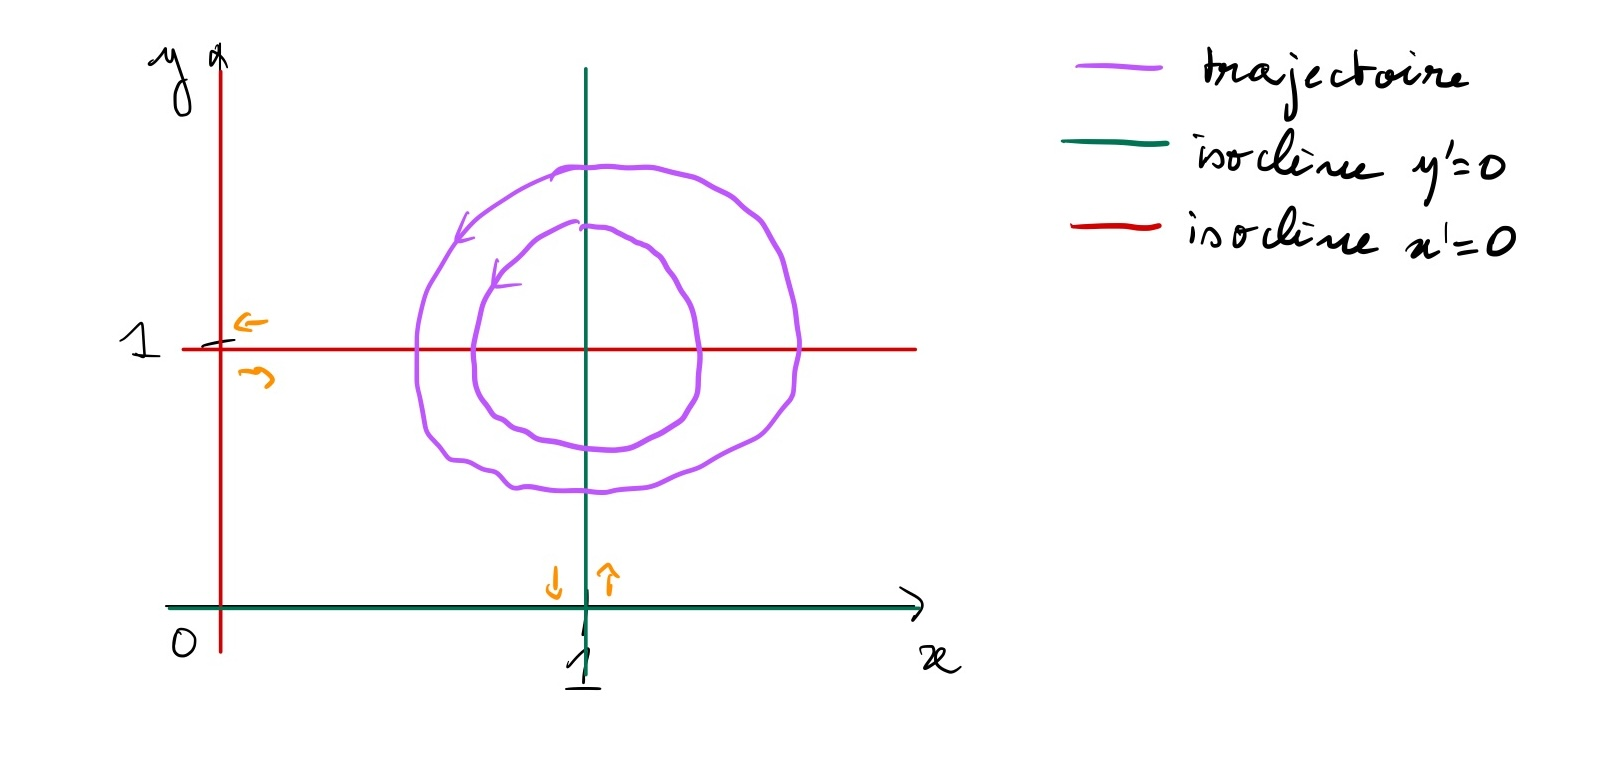
\includegraphics[width=0.5\textwidth]{portrait_phase.jpg}
      \item si on part du cadran nord ouest, $x$ et $y$ sont décroissants. Si on reste dans ce cadran, $x$ et $y$ tendent vers une limite, or par passage à la limite dans l’EDO, les seuls points stables sont $(0,0)$ et $(1,1)$ contradiction.
      Donc on passe dans le cadran sud-ouest. Par un raisonnement similaire, on fait le tour.
      \item quand on revient, on doit repasser par le même point (parce que $H$ est monotone là où il faut)
    \end{enumerate}
  \end{enumerate}
\end{solution}

\newpage
\section*{Correction exercice d’optimisation}

\begin{solution}
 \begin{enumerate}
  \item $S$ définit un produit scalaire, donc l’ensemble admissible est fermé, borné et $f$ est continue donc le problème admet une solution 
  \item Calcul direct.
  \item Les équations d’Euler Lagrange nous disent qu’une solution du problème d’optimisation sous contrainte s’écrit 
  \[
    \nabla f(x) + \lambda g(x)=0.  
  \]
  \item $B = L^{-T} A L^T$.
  \item on a $\lambda = \langle x, A x \rangle = f(x)$ par la contrainte, donc la solution est donnée par un vecteur propre associé à la plus petite vp de $B$.
   On a unicité que si la plus petite vp de $B$ est de multiplicité 1.
   \item $S$ est SDP et $J_\mu$ est quartique
   \item par coercivité et continuité de $J_\mu$
   \item on a $p(x_*) = 0$ et par optimalité de $x_\mu$, nécessairement $J_\mu(x_\mu) \leq J(x_*)$.
   \item \begin{enumerate}
    \item par définition des $x_{\mu}$
    \item en additionnant les deux équations. Si $p(x_{\mu_n}) = P>0$, $J_{\mu_n}(x_{\mu_n})$ tend vers l’infini ce qui contredit Q8.
    \item en passant à la limite, $\overline{x}$ satisfait la contrainte et $J(\overline{x}) \leq J(x_*)$ donc $\overline{x} = x_*$ par unicité du minimiseur.
   \end{enumerate}
 \end{enumerate} 
\end{solution}

\end{document}
